% Plantilla TFG LaTeX LSI por:
%   Agustín Borrego <borrego@us.es>
%   Inma Hernández <inmahernandez@us.es>
% Su uso y modificación es libre.

% ̀¡Recuerda hacer copias de seguridad frecuentes durante la redacción del trabajo!
% Puedes descargar todo el código fuente del proyecto en zip en Menú > (Descargar) Fuente

\documentclass[12pt]{report}

% Paquetes LaTeX y estilos globales
\usepackage[utf8]{inputenc}
\usepackage{multicol}
\usepackage{xcolor}
\usepackage{subfigure}
\usepackage[spanish,es-tabla]{babel}
\usepackage[utf8]{inputenc}
\usepackage{graphicx}
\usepackage{titlesec}
\usepackage[bookmarks,breaklinks,colorlinks=true,allcolors=blue]{hyperref}
\usepackage{listings}
\usepackage{inconsolata}
\usepackage{float}
\usepackage{mathpazo} % Fuente Palatino
\usepackage[labelfont=bf]{caption}

\usepackage[square,numbers]{natbib}
\usepackage[nottoc,notlof,notlot]{tocbibind}  % Mete la bibliografía como capítulo en la TOC, los parámetros excluyen los otros índices de aparecer también
\usepackage{geometry}
\usepackage{amsmath}
\usepackage{parskip}
\usepackage[official]{eurosym}
\usepackage{todonotes}
\usepackage{csquotes}
\usepackage{tocbasic}  % Estilos de la TOC

% Formato del título de capítulos y secciones
\titleformat{\chapter}[block]{\normalfont\huge\bfseries}{\thechapter.}{.5em}{\Huge}[\vspace{2pt}{\titlerule[2pt]}]

\titlespacing*{\chapter}{0pt}{-19pt}{25pt}

\titleformat{\section}[block]{\normalfont\Large\bfseries}{\thesection.}{.5em}{\Large}

\titleformat{\part}[block]{\titlerule[2pt]\normalfont\Huge\bfseries\centering}{Parte \Roman{part}\\\vspace{15pt}}{0pt}{\Huge}[\vspace{2pt}{\titlerule[2pt]}]

% Tamaños y estilos de elementos en la TOC
\DeclareTOCStyleEntry[
    linefill=\bfseries\TOCLineLeaderFill,
    beforeskip=12pt,
    entrynumberformat=\chapterprefixintoc,
    entryformat=\chaptertocformat,
    pagenumberformat=\chaptertocformat,
    dynnumwidth
]{tocline}{chapter}

\DeclareTOCStyleEntry[
    % linefill=\bfseries\TOCLineLeaderFill,
    beforeskip=30pt,
    entrynumberformat=\chapterprefixintoc,
    entryformat=\parttocformat,
    pagenumberformat=\partpagetocformat,
    numwidth=0pt
]{tocline}{part}

\newcommand\chaptertocformat[1]{\large{\textbf{#1}}}%
\newcommand\chapterprefixintoc[1]{#1}%
\newcommand\parttocformat[1]{\Large{\textbf{#1}}}%
\newcommand\partpagetocformat[1]{} % Don't print the page number for parts

% Alias para estilos de texto comunes
\newcommand{\negritas}[1]{\textbf{#1}}
\newcommand{\cursiva}[1]{\textit{#1}}
\newcommand{\codigo}[1]{\texttt{#1}}

% Formato del código fuente con lstlisting
\lstset{
  basicstyle=\ttfamily,
  breaklines=true,
}

% Márgenes
\geometry{
    a4paper,
    margin=2.75cm
}
\setlength{\marginparwidth}{2cm} 

% Limite de profundidad del índice
\setcounter{tocdepth}{2}

% Eliminar el guionado
\tolerance=1
\emergencystretch=\maxdimen
\hyphenpenalty=10000
\hbadness=10000

% Indentación de párrafos
\setlength{\parindent}{.75cm}

\renewcommand{\lstlistingname}{Extracto de código}
\renewcommand*{\lstlistlistingname}{Índice de extractos de código}

% Comandos para establecer variables
\newcommand{\setTitle}[1]{\def\tfgTitle {#1}}
\newcommand{\setAuthor}[1]{\def\tfgAuthors {#1}}
\newcommand{\setDegree}[1]{\def\tfgDegree {#1}}
\newcommand{\setSupervisor}[1]{\def\tfgSupervisor {#1}}
\newcommand{\setDepartment}[1]{\def\tfgDepartment {#1}}
\newcommand{\setMonth}[1]{\def\tfgMonth {#1}}
\newcommand{\setYear}[1]{\def\tfgYear {#1}}
\newcommand{\setDedication}[1]{\def\tfgDedication {#1}}

% Estilos para el código
% Configuración genérica
\definecolor{codegreen}{rgb}{0,0.6,0}
\definecolor{codegray}{rgb}{0.5,0.5,0.5}
\definecolor{codepurple}{rgb}{0.58,0,0.82}
\definecolor{editorOcher}{rgb}{0.8, 0.3, 0} % #FF7F00 -> rgb(239, 169, 0)
\definecolor{editorGreen}{rgb}{0, 0.5, 0} % #007C00 -> rgb(0, 124, 0)

\lstdefinestyle{listingstyle}{
    backgroundcolor=\color{white},  
    keywordstyle=\bfseries\color{blue},
    numberstyle=\tiny\color{codegray},
    stringstyle=\color{editorGreen},
    commentstyle=\color{codegray},
    basicstyle=\ttfamily\color{black},
    breakatwhitespace=false,         
    breaklines=true,                 
    captionpos=b,                    
    keepspaces=true,                 
    numbers=left,                    
    numbersep=5pt,                  
    showspaces=false,                
    showstringspaces=false,
    showtabs=false,                  
    tabsize=2,
    frame=tb,
    keywords=[2]{True,False},
    literate=%
*{0}{{{\color{editorOcher}0}}}1
{1}{{{\color{editorOcher}1}}}1
{2}{{{\color{editorOcher}2}}}1
{3}{{{\color{editorOcher}3}}}1
{4}{{{\color{editorOcher}4}}}1
{5}{{{\color{editorOcher}5}}}1
{6}{{{\color{editorOcher}6}}}1
{7}{{{\color{editorOcher}7}}}1
{8}{{{\color{editorOcher}8}}}1
{9}{{{\color{editorOcher}9}}}1,
}

\lstset{style=listingstyle}
\lstset{columns=fullflexible}

\lstdefinelanguage{css}{
  keywords={color,background-image:,margin,padding,font,weight,display,position,top,left,right,bottom,list,style,border,size,white,space,min,width, transition:, transform:, transition-property, transition-duration, transition-timing-function},	
  sensitive=true,
  morecomment=[l]{//},
  morecomment=[s]{/*}{*/},
  morestring=[b]',
  morestring=[b]",
  alsoletter={:},
  alsodigit={-}
}
% JavaScript
\lstdefinelanguage{javascript}{
  morekeywords={abstract, arguments, await, boolean, break, byte, case, catch, char, class, const, continue, debugger, default, delete, do, double, else, enum, eval, export, extends, false, final, finally, float, for, function, goto, if, implements, import, in, instanceof, int, interface, let, long, native, new, null, package, private, protected, public, return, short, static, super, switch, synchronized, this, throw, throws, transient, true, try, typeof, var, void, volatile, while, with, yield},
  morecomment=[s]{/*}{*/},
  morecomment=[l]//,
  morestring=[b]",
  morestring=[b]'
}

%Para quitar la sangría al principio de cada párrafo
\setlength{\parindent}{0pt}
%Para dar formato al indice de los enumerados
\usepackage{enumitem}
%Establece el formato ''code'' para código
\newcommand{\code}[1]{\texttt{\textsc{#1}}}
%Para mostrar un encabezado con el capítulo al que pertenece la página
\usepackage{fancyhdr}
\pagestyle{fancy}
\fancyhf{}
\fancyhead[LE,RO]{\slshape \leftmark} %rigthmark muestra la subsec
\fancyfoot[C]{\thepage}
%


%%%%%%%%%%%%%%%%%%%%%%%%%%%%%%%%%%%%%%%%%%%%%%%%%%%%%%%%%%%%%%%%%%%%%%%%%%%%%%%%%%%%%

% Variables para la portada
\setTitle{Despliegue de Broadsea para la estandarización con ATLAS de un estudio clínico convertido a OMOP CDM
}
%Extrayendo conocimiento a partir de análisis clínico de datos CDM usando la herramienta Atlas

%%%%%%%% {Estandarización de estudio clínico oncológico mediante OMOP CDM y análisis a través de ATLAS Broadsea





\setAuthor{Da. María del Valle Alonso de Caso Ortiz} % Si hay más de un autor, separarlos con \\
\setDegree{Grado en Ingeniería de la Salud} % Cambiar si es necesario
\setSupervisor{Dr. Julián Alberto García García \\ Dra. María José Escalona Cuaresma} % Si hay más de un tutor, separarlos con \\
\setDepartment{Lenguajes y Sistemas Informáticos}
\setMonth{junio} % Dejar sólo el mes de la convocatoria en que se presenta el trabajo
\setYear{2023/24} % Por ejemplo, 2022/23

%%%%%%%%%%%%%%%%%%%%%%%%%%%%%%%%%%%%%%%%%%%%%%%%%%%%%%%%%%%%%%%%%%%%%%%%%%%%%%%%%%%%%

% Dedicatoria del trabajo
% Si no se desea incluir, comentar o borrar la línea siguiente para eliminar la página de dedicatoria
\setDedication{A mi padre y a mi madre, por inculcarme la pasión por el estudio y acompañarme incondicionalmente en cada etapa del camino.}

%%%%%%%%%%%%%%%%%%%%%%%%%%%%%%%%%%%%%%%%%%%%%%%%%%%%%%%%%%%%%%%%%%%%%%%%%%%%%%%%%%%%%

% Comienzo del documento
\begin{document}

    % Portada y secciones no numeradas
    \thispagestyle{empty} % Impide que se incluya número de página en la portada
\begin{center}

\vspace*{1cm}


\includegraphics[width=\textwidth]{figures/etsii_us.png}

\vspace*{2.5cm}
\begin{large}
TRABAJO FIN DE GRADO
\end{large}

\vspace*{0.1in}
\textbf{\huge \tfgTitle}

\vspace*{.5in}

{\large Realizado por}\\
\textbf{\Large \tfgAuthors}

\vspace*{2cm}

\textbf{Para la obtención del título de}\\
{\large \tfgDegree}

\vspace*{0.2in}

\textbf{Dirigido por}\\
{\large \tfgSupervisor}\\

\vspace*{0.2in}

\textbf{En el departamento de}\\
{\large \tfgDepartment}

\vspace*{.6in}
\textbf{\Large Convocatoria de \tfgMonth, curso \tfgYear}

\end{center}

% Dedicatoria
\ifdefined\tfgDedication
    \newpage
    \thispagestyle{empty}
    
    \vspace*{\fill}
    \begin{center}
    \textit{\tfgDedication}
    \end{center}
    \vspace*{\fill}
\fi

\clearpage\setcounter{page}{1} % Comienza a incluir números de página a partir de aquí
\pagenumbering{roman} % En números romanos
    \chapter*{Agradecimientos}


    \chapter*{Resumen}
Incluya aquí un resumen de los aspectos generales de su trabajo, en español.

\vspace{.5cm}

\textbf{Palabras clave:} Palabra clave 1, palabra clave 2, ..., palabra clave N
    \chapter*{Abstract}
This section should contain an English version of the Spanish abstract.

\vspace{.5cm}

\textbf{Keywords:} Keyword 1, keyword 2, ..., keyword N
    
    % Índice del documento y de figuras
    \begingroup
        % Los enlaces son normalmente azules, pero en los índices se configuran a negro para que no aparezca todo azul
        \hypersetup{linkcolor=black}
        \tableofcontents
        \listoffigures
        \listoftables
        \lstlistoflistings
    \endgroup
    
    % Cambia el estilo de números de página de romanos a normal
    \clearpage\pagenumbering{arabic}
    
    % Capítulos del trabajo
    %\chapter{Ejemplos de uso de LaTeX}\label{cap:ejemplos}

\todo[inline]{Este capítulo se incluye únicamente como ayuda y referencia de uso de \LaTeX. No debe aparecer en el documento final.}

\section{Introducción}
En este capítulo se muestran ejemplos de uso de \LaTeX{} para operaciones comunes. 

\section{Estilos}\label{sec:estilos}
Se pueden aplicar estilos al texto como \textbf{negritas}, \textit{cursiva}, \underline{subrayado} y \texttt{monoespaciado}. También se \textcolor{red}{pueden} \textcolor{blue}{aplicar} \textcolor{green}{colores}, y \underline{\textit{combinar}} \textbf{\textcolor{red}{estilos}}. Se recomienda usar sólo negritas para hacer énfasis, y no abusar de este recurso.

Por comodidad para usuarios no habituados con LaTeX, esta plantilla define algunos alias de comandos más fáciles de recordar para estilos de texto comunes: \negritas{negritas}, \cursiva{cursiva} y \codigo{código}.

\section{Listados}
Con itemize se pueden crear listas no numeradas:

\begin{itemize}
    \item Fresas
    \item Melocotones
    \item Piñas
    \item Nectarinas
\end{itemize}

De manera similar, enumerate permite crear listas numeradas:

\begin{enumerate}
    \item Elaborar la memoria del TFG
    \item Elaborar la presentación
    \item Presentar el TFG
    \item Solicitar el título de Grado
\end{enumerate}

\section{Subsecciones}
Se pueden definir subsecciones con el comando \texttt{subsection}:

\subsection{Primera subsección}\label{sec:subseccion}
Esto es una subsección

\subsection{Segunda subsección}
Esto es otra subsección.

\subsubsection{Sub-sub-sección}
Este es un tercer nivel de profundidad, que no aparece en el índice general. Se recomienda no utilizarlo, si es posible.

\section{Imágenes y figuras}
Todas las imágenes y figuras del documento se incluirán en la carpeta ``figures''. Se pueden incluir de la siguiente manera:

\begin{figure}[htp]
    \centering
    
\includegraphics[width=0.7\textwidth]{figures/ejemplo.png}
    \caption{Un feroz depredador}
    \label{fig:ejemplo}
\end{figure}

Observe que las figuras se numeran automáticamente según el capítulo y el número de figuras que hayan aparecido anteriormente en dicho capítulo. Existen muchas maneras de definir el tamaño de una figura, pero se aconseja utilizar la mostrada en este ejemplo: se define el ancho de la figura como un porcentaje del ancho total de la página, y la altura se escala automáticamente. De esta manera, el ancho máximo de una figura sería 1.0 * textwidth, lo que aseguraría que se muestra al máximo tamaño posible sin sobrepasar los márgenes del documento.

Tenga en cuenta que LaTeX intenta incluir las figuras en el mismo sitio donde se declaran, pero en ocasiones no es posible por motivos de espacio. En esos casos, LaTeX colocará la figura lo más cerca posible de su declaración, puede que en una página diferente. Esto es un comportamiento normal.

\section{Tablas}
Existe una gran variedad de formas de crear tablas en LaTeX puro, y todas ellas tienen cierta complejidad. A continuación se muestra un ejemplo simple de tabla nativa, en la Tabla \ref{table:ejemplo}. Se recomienda crear un archivo en la carpeta \textit{tables} por cada tabla nativa que se desee incluir, y enlazarla mediante el comando \texttt{input}.

\begin{table}[htp]
\centering

    % Esta primera línea define las columnas de la tabla. Los posibles tipos de columna son:
    % c: texto centrado
    % l: texto alineado a la izquierda
    % r: texto centrado a la derecha
    % p: columna de ancho fijo
    % Las columnas tienen ancho dinámico según la anchura máxima de los elementos que contengan.

    % Las columnas l/r/c no parten el texto en filas diferentes si éste es demasiado largo. Para ello, puede utilizar el tipo de columna de ancho fijo "p".
    
    % Las barras verticales | se usan para definir los bordes verticales de la tabla. Pruebe a eliminar algunas y observe qué ocurre.
    \begin{tabular}{ | l | c | r | p{2cm} | }
        
        % A continuación van las filas de la tabla. En cada fila, las columnas se separan con el carácter &
        % Para terminar una fila se usa \\
        % Para incluir un borde horizontal entre filas se usa \hline

        % Cabecera con textos en negrita:
        \hline
        \textbf{Columna L} & \textbf{Columna C} & \textbf{Columna R} & \textbf{Columna P}\\
        \hline
        
        % Cuerpo de la tabla:
        Texto de ejemplo & Texto de ejemplo & Texto de ejemplo & Texto de ejemplo\\
        \hline
        ABC & DEF & HIJ & KLM\\
        \hline
        
    \end{tabular} 
    
    \caption{Tabla LaTeX de ejemplo}
    \label{table:ejemplo} 
\end{table}


Para tablas con un formato más complejo, considere la posibilidad de diseñarla usando otro software externo (por ejemplo Excel) e incluirla de manera similar a una figura. \textbf{Observe en el código LaTeX a continuación cómo usar el comando \texttt{captionof\{table\}}, en lugar de simplemente \texttt{caption}, hace que se liste como una Tabla en lugar de como una Figura}:

\begin{figure}[htp]
    \centering
    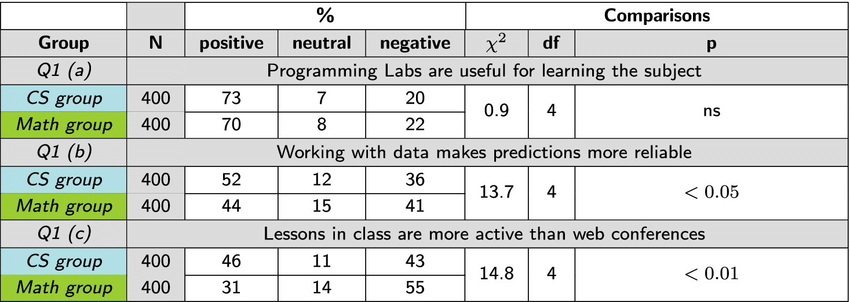
\includegraphics[width=1.0\textwidth]{tables/complex_table.png}
    \captionof{table}{Tabla compleja introducida como figura}
    \label{table:ejemplo2}
\end{figure}

\section{Referencias}
Observe cómo en el código fuente de esta sección se ha usado varias veces el comando \texttt{label}. Este comando permite marcar un elemento, ya sea capítulo, sección, figura, etc. para hacer una referencia numérica al mismo. Para referenciar una label se usa el comando \texttt{ref} incluyendo el nombre de la referencia:

Este es el capítulo \ref{cap:ejemplos}.

En la sección \ref{sec:estilos} se muestran ejemplos de estilos.

La subsección \ref{sec:subseccion} explica...

En la Figura \ref{fig:ejemplo} vemos que...

Esto evita que tengamos que escribir directamente los índices de las secciones y figuras que queremos mencionar, ya que LaTeX lo hace por nosotros y además se encarga de mantenerlos actualizados en caso de que cambien (pruebe a mover este capítulo al final del documento y observe cómo se actualizan automáticamente todos los índices referenciados). Además, las referencias mediante ``ref'' actúan como hipervínculos dentro del documento que llevan al elemento referenciado al pulsar en ellas.

Es habitual nombrar las ``label'' con un prefijo que indica el tipo de elemento para encontrarlo luego más fácilmente, pero no es obligatorio.

\section{Extractos de código}

Se pueden incluir extractos de código mediante lstlisting:

\begin{lstlisting}[language=Python, caption={Código Python}, label={cod:python}, captionpos=b]
num = float(input("Enter a number: "))
if num > 0:
   print("Positive number")
elif num == 0:
   print("Zero")
else:
   print("Negative number")
\end{lstlisting}

Para evitar tener que incluir el código directamente en el texto del documento, se pueden guardar en archivos separados y referenciarlos:

\lstinputlisting[
    float,
    floatplacement=!htp,
    language=Java,
    label=cod:java,
    caption=Código Java
]{code/java_example.java}

\lstinputlisting[
    float,
    floatplacement=!htp,
    language=html,
    label=cod:html,
    caption=Código HTML
]{code/html_example.html}

\lstinputlisting[
    float,
    floatplacement=!htp,
    language=javascript,
    label=cod:js,
    caption=Código JavaScript
]{code/javascript_example.js}

Los extractos de código también se pueden referenciar mediante label/ref: Extractos de código \ref{cod:python}, \ref{cod:java}, \ref{cod:html}, \ref{cod:js}. 

\section{Enlaces}
Puede enlazar una web externa mediante el comando \texttt{url}: \url{https://www.example.com}. También se puede vincular un enlace a un texto mediante el comando href: \href{https://www.example.com}{dominio de ejemplo}.

\section{Citas y bibliografía}
En LaTeX, los elementos de la bibliografía se almacenan en un fichero bibliográfico en un formato llamado BibTeX, en el caso de este proyecto se encuentran en ``bibliografia.bib''. Para citar un elemento se usa el comando \texttt{cite}. Se pueden citar tanto artículos científicos \cite{borrego2019} como enlaces web \cite{webETSII}. 

También se puede usar el comando \texttt{citet} para incluir una referencia junto con el nombre de su autor o autores: \citet{borrego2021}. Todas las citas se numeran automáticamente y se incluyen en la sección de bibliografía del trabajo. El orden por defecto es según su orden de aparición en el documento. Para ordenarlas por orden alfabético del autor, puede modificar el comando \texttt{bibliographystyle} del archivo principal y reemplazar su valor por el estilo \texttt{plainnat} (orden alfabético, nombres completos) o \texttt{abbrvnat} (orden alfabético, nombres abreviados).

Observe cómo los elementos bibliográficos almacenados en ``bibliografia.bib'' tienen una etiqueta asociada, que es la que se usa al citarlos mediante cite. \textbf{Añadir una referencia al fichero bibliográfico no hace que ésta aparezca automáticamente en la sección de bibliografía del trabajo, es necesario citarla en algún lugar del mismo}.

\section{Ecuaciones}
LaTeX tiene un potente motor para mostrar ecuaciones matemáticas y un amplio catálogo de símbolos matemáticos. El entorno matemático se puede activar de muchas maneras. Para incluir ecuaciones simples en un texto se pueden rodear de símbolos dólar: $1 + 2 = 3$, $\sqrt{81} = 3^2 = 9$, $\forall x \in y~\exists~z : S_z < 4$.

Las ecuaciones más complejas pueden expresarse aparte y son numeradas: ecuación \ref{eq:ecuacion}.

\begin{equation}\label{eq:ecuacion}
\lim_{x\to 0}{\frac{e^x-1}{2x}}
 \overset{\left[\frac{0}{0}\right]}{\underset{\mathrm{H}}{=}}
 \lim_{x\to 0}{\frac{e^x}{2}}={\frac{1}{2}}
 +7 \int_0^2
  \left(
    -\frac{1}{4}\left(e^{-4t_1}+e^{4t_1-8}\right)
  \right)\,dt_1
\end{equation}

Dispone \href{http://www.yann-ollivier.org/latex/texsymbols.pdf}{aquí} de un amplio listado de símbolos que pueden usarse en modo matemático.

\section{Caracteres y símbolos especiales}
Algunos caracteres y símbolos deben ser escapados para poder representarse en el documento, ya que tienen un significado especial en LaTeX. Algunos de ellos son:

\begin{itemize}
    \item El símbolo dólar \$ se usa para ecuaciones.
    \item El tanto por ciento \% se usa para comentarios en el código fuente.
    \item El símbolo euro \euro{} suele dar problemas si se escribe directamente.
    \item El guión bajo \_ se usa para subíndices en modo matemático.
    \item Las comillas deben expresarse `así' para comillas simples y ``así'' para comillas dobles. Las comillas españolas pueden expresarse \textquote{así}.
    \item La barra invertida o contrabarra \textbackslash{} se usa para comandos LaTeX.
    \item Otros símbolos que deben escaparse son las llaves \{ \}, el ampersand \&, la almohadilla \# y los símbolos mayor que \textgreater{} y menor que \textless{}.
\end{itemize}
    \chapter{Introducción, Contexto y Motivación}\label{cap:introduccion}

%Este apartado tiene un tono un poco más personal,
%al fin y al cabo relata mi vivencia y opinión subjetiva sobre el TFG

\section{Introducción}

En palabras de Malcom X, \textit{"la educación es el pasaporte hacia el futuro, ya que el mañana pertenece a aquellos que se preparan para el hoy"}, y tanto es así que han sido cuatro años de preparación y dedicación día a día los que me han ido formando personal y académicamente hasta alcanzar la realización de este Trabajo de Fin de Grado, que abre las puertas de mi futuro profesional.

%%MODIFICACIÓN--------------------------------------
En esta primera sección se presenta el contexto y la motivación que trascienden a la realización del Trabajo.
%%MODIFICACIÓN-------------------------------------------


\section{Contexto // por el que se selecciona este topico //}



%Los tiempos que corren ahora son tiempos cambiantes, Industria 4.0, el auge de las IA, la importancia de la interoprerabilidad y los estándares... 

%- Propuestas a nivel europeo? OHDSI?


%- Hablar de OHDSI EN SEVILLA

%    [Innodata2023]
    
%- La selección de este tópico se debe al creciente interés por el estándar de OHDSI en Sevilla (Hospital Macarena y/o Hospital V del Rocio) y en España.

%- Comentar Aplicaciones reales y actuales del estandar. Además del interés a nivel mundial (Ohdsi en Europa Y en america del norte). Ohdsi community.
    


\section{Motivación}

%Mi motivación personal de entrar en el mundo del %análisis de datos clínicos utilizando  esta %herramienta prometedora..






    








    \chapter{Objetivos del proyecto}\label{cap:objetivos}

\section{Objetivos del TFG}

- Extraer evidencia relevante a partir de datos clínicos observacionales


\section{Objetivos Personales}

- Aumentar mi conocimiento del estándar de OHDSI

- AUmentar mi experiencia en el manejo de datos clínicos

- Aumentar mi conocimeinto en el mundo de análisis de datos

    \chapter{Gestion del Proyecto}\label{cap:gestión}

\section{Introducción}
Breve introducción al capítulo

\section{Participantes del Proyecto}

- Yo M.V ALONSO
- Julian
- M. Jose 

%\section{Estructura de desglose de trabajo}


\section{Estimación de recursos}

- PC, licencias windows, office; recursos open-source de OHDSI a través de youtube, github, docker...

\section{Planificación temporal}

- Scrum, planificación por sprints, estimación del tiempo, desviación...

\section{Evaluación de costes}

- PC, licencias windows, office, teams, ATLAS, OHDSI; gastos indirectos (luz)...

%\section{Identificación de riesgos y planes de contingencia}


    \chapter{Metolodología}\label{cap:metodologia}

Metodología usada para la gestión del proyecto

- Scrum

- sofIA???

\textbf{Este apartado se podría incluir en el capitulo 3-Gestion, concretamente cuando se expone la planificación temporal}
    
    \chapter{Estudio Previo}\label{cap:estudio}

\section{Introduccion}

En esta sección se muestra un estudio comprensivo del estandar OHDSI utilizado: qué es, su ......

\section{Qué es OHDSI}

Observational Health Data Science and Informatics

....

\subsection{Historia}

Surgimiento a partir del proyecto OMOP

\subsection{Misión, Visión y Valores}

-
-
-

\subsection{Red colaborativa}

- Collaborative network across XX countries, organizations...
- Github....
- Community calls...
-Symposium

\section{Cómo generar evidencia}

- A journey from data to evidence (buscar en la documentación de ohdsi)

\subsection{Building blocks of OHDSI}

(buscar en la documentación de ohdsi)

\subsection{Estandarización de los datos}

- OMOP CDM

- OMOP VOCABULARY

\subsection{Investigación metodológica}
%%ADEMAS DE SER LOS TRES MÉTODOS QUE OFRECE OHDSI PARA REALZIAR INVESTIGACIONNES SON 3 CASOS DE USOS
-Caracterizacion
-Estimacion a nivel de poblacion
-Prediccion a nivel de paciente

\section{Herramientas}
\subsection{ATLAS}

- Extensa descripción de ATLAS (versión actual, anteriores, uso, aspecto...)

ATLAS ADEMÁS IMPLEMENTA INTRÍNSICAMENTE  DOS HERRAMIENTAS

-ATHENA (herramienta de busqueda en el vocabulario del CDM) actualemnte está implementada dentro de ATLAS/Search

- ACHILLES (data quality dashboard) también esta implementada actualmente dentro de ATLAS/Data source


\subsection{Otras herramientas}

breve descripción de cada una:

-HADES (herramientas de análisis pero en librerias R)

-WHITE-RABBIT y RABBIT-IN-A-HAND (para preparar las ETL)

USAGI (también para la ETL)
...

\section{Conclusiones}

    
    \chapter{Documento de Requisitos}\label{cap:requisitos}

\section{Introducción}


%R.I%%%%%%%%%%%%%%%%%%%%%%%%%%%%%%%%%%%%%%%%%%%%%%%%%%%%%%%%%%%%%%%%%%%%%
%\section{Requisitos de Información}


%R.F%%%%%%%%%%%%%%%%%%%%%%%%%%%%%%%%%%%%%%%%%%%%%%%%%%%%%%%%%%%%%%%%%%%%%
\section{Requisitos Funcionales}

- RF00: Cargar datasets //De hecho este aún no sabemos como hacerlo. Estamos trabajando con datasets que ya vienen cargados

- RF01: Obtener un reporte del data set (Data source)

- RF02 : Definir un conjunto de conceptos del Vocabulario (Concept set)

- RF03: Configurar la muestra de trabajo (cohort definition)

- RF04: Caracterizar el cohort (characterization - primer gran bloque de metodología de OHDSI)

- RF05: Definir una etsimacion a nivel de poblacion (estimation - segundo gran bloque de metodologia de OHDSI)

- RF06: Hacer una prediccion a nivel de paciente (prediction - tercer gran bloque de metodologia de OHDSI)



Más cosas que se pueden hacer y no definimos la otra vez:

- Obtener un reporte de la ruta del cohorte (cohort pathway)

- Analizar los ratios de incidencia de un outcome (INcidence rate)

- Obteenr un reporte de los datos para un paciente concreto (profile)

\subsection{Diagramas de casos de uso}


\subsection{Descripción del requisito}


%\subsection{Diagramas de casos de uso}
%\subsection{¿¿¿¿¿Descripción del requisito funcional????}


%\section{Modelo conceptual}%%%%%%%%%%%%%%%%%%%%%%%%%%%%%%%%%%%%%%%%%%%%%%

%\section{Mockups}%%%%%%%%%%%%%%%%%%%%%%%%%%%%%%%%%%%%%%%%%%%%%%%%%%%%%%%%

%R.N.F%%%%%%%%%%%%%%%%%%%%%%%%%%%%%%%%%%%%%%%%%%%%%%%%%%%%%%%%%%%%%%%%%%%%
\section{Requisitos no Funcionales}





\section{Conclusiones}
En este capítulo concluimos que...


    \chapter{Documento de Análisis y Diseño}\label{cap:diseño}

\section{Introducción}
En este capítulo explicaremos...

\section{Arquitectura del Sistema}

Todo el sistema de OHDSI con todas sus herramientas se organiza...

Ampliamente
- Plataforma open-source en github: toda la info y código de todo se encuentra aqui


Concretamente para este trabajo,
se ha usado el "subssistema" de
- OHDSI BROADSEA APPLICATIONS con la base de datos de EUNOMIA

*Se podría extender a más bases de datos pero aún no sabemos cómo hacerlo

- Implementado en el ordenador personal usando DOCKER







%\section{Modelo de Persistencia}

%\section{Diagrama de Componentes}

%\section{Entorno tecnológico}

\section{Conclusiones}
En este capítulo concluimos que...

    \chapter{Plan de pruebas}\label{cap:pruebas}
%%%%%%%%%%%%%%%55

Este capítulo podría ser más bien "Casos prácticos"

\section{Introducción}

\section{Casos prácticos}

%\section{Pruebas Unitarias}
%\section{Pruebas de Integración}
%\section{Pruebas de Carga o Rendimiento}
%\section{Pruebas Funcionales}

Mostrar un ejemplo práctico utilizando ATLAS para cada caso de uso,

ej de la obtención dle reporte de la BD,
ej de la creación de un cohorte concreto para un estudio concreto,
ej de la predicción a nivel de paciente para un estudio concreto....

todos los ejemplos anteriores seguirían un mismo hilo conductor en cuanto al ESTUDIO CONCRETO

\section{Conclusiones}

En este capítulo concluimos que...

    \chapter{Resultados}\label{cap:resultados}

\section{Lecciones aprendidas}

- Comprensión de la importancia de la estandarización (estandar OHDSI) en la interoperabilidad de los sistemas clínicos.

- Implementación de un entorno virtual en el PC (Entorno y webAPI de OHDSI en MV DOCKER)

- Aprendizaje de uso de la herramienta ATLAS

...

\section{Trazabilidad de objetivos}

    %\chapter{¿¿¿¿Implementación??????}\label{cap:implementacion}

\section{Introducción}
En este capítulo explicaremos...

\section {Herramientas}

\section{Conclusiones}
En este capítulo concluimos que...

    \chapter{Conclusiones}\label{cap:conclusiones}




    \bibliographystyle{unsrtnat}
    \bibliography{bibliografia.bib}


    \appendix
    \chapter{Manual de ATLAS Broadsea}\label{anexo:manual}

El nombre completo de este anexo corresponde a \textbf{Manual de instalación, despliegue y configuración de ATLAS Broadsea}, aunque por motivos de extensión se ha reducido en el índice de la memoria a \textit{Manual de ATLAS Broadsea}.

El manual se presenta a la convocatoria como un documento aparte debido a su larga extensión, de casi 40 páginas. No obstante, se utiliza este apartado de la memoria para presentar resumidamente sus contenidos básicos y cómo acceder a él. Su gran extensión se debe a a que recopila en un único lugar una grandísima variedad de información que hasta ahora se encontraba esparcida de forma más o menos ordenada en la red, sobretodo en diferentes repositorios de github. 

El anexo se adjunta a la documentación entregable de la convocatoria con el nombre ''Anexo A - Manual de ATLAS Broadsea.pdf''. Adicionalmente, también es accesible a través del repositorio de github del Trabajo Fin de Grado \cite{vallealonsodc}, concretamente en la ruta \code{Thesis-ATLAS-OHDSI/documentation/pdf}.

%El manual es un documento de gran valor debido a que recopila en un único lugar una grandísima variedad de información que hasta ahora se encontraba esparcida de forma más o menos ordenada en la red, pero nunca recopilada en un único documento. Su redacción como un documento aparte nace de la propia dificultad a la que se enfrenta la alumna a la hora de instalar, desplegar y configurar la herramienta para la reproducción del estudio práctico con el fin de facilitar a futuros usuarios y a sus propios compañeros del departamento de Innovación Tecnológica del Hospital Universitario Virgen del Rocío una guía detallada con todos los contenidos necesarios para replicar esta tarea cuando fuere necesario.

El manual trata cinco aspectos importantes de ATLAS Broadsea: 

\begin{enumerate}
    \item \textbf{Introducción y descripción de Broadsea.} Este capítulo explica contenidos sobre el entorno tecnológico necesario para seguir correctamente los procedimientos del manual.
    \item \textbf{Despliegue por defecto.} Este capítulo presenta el despliegue más sencillo del entorno Broadsea, sin ningún tipo de configuración adicional.
    \item \textbf{Conexión con la BD por defecto.} Este capítulo explica la conexión con el servidor Postgre del contenedor docker de Broadsea.
    \item \textbf{Conexión con BD externa.} Este capítulo explica cómo añadir una conexión de una base de datos externa al servidor docker de Broadsea.
    \item \textbf{Configuración del Vocabulario.} Eeste capítulo explica cómo configurar el Vocabulario desde ATHENA y se presentan otras configuraciones avanzadas.
\end{enumerate}

Todo ello complementa la información del TFG de forma subyacente, es decir, durante la reproducción del estudio práctico (véase \ref{cap:08pruebas}) se da por supuesto todo el proceso de instalación de la herramienta así como la configuración del servidor, base de datos, étc. En términos de roles del proyecto (véase \ref{cap:03gestión}) se podría decir que mientras que el analista se encarga de reproducir el estudio haciendo uso de la interfaz de usuario de ATLAS, el developer habría sido el encargado de realizar toda el anexo, con toda la instalación, despliegue y configuración para que la herramienta funcione. No obstante, en este caso ambos roles son ejecutados por la misma persona que es la alumna. Además satisface explícitamente el \textbf{Obj-002} del Trabajo Fin de Grado (véase \ref{cap:02objetivos}).




    \chapter{Glosario}\label{anexo:glosario}


\textbf{Aprendizaje automático (\textit{Machine Learning, ML}):} Campo de la inteligencia artificial que desarrolla algoritmos y modelos que permiten a las máquinas aprender a partir de datos, identificar patrones y tomar decisiones sin necesidad de ser programadas explícitamente para cada tarea específica.

\textbf{ATLAS}: Herramienta de código abierto desarrollada por la colaboración Observational Health Data Sciences and Informatics (OHDSI), diseñada para la visualización, exploración y análisis de datos de salud provenientes de diferentes fuentes y estándares, facilitando la investigación en salud pública y la toma de decisiones clínicas basadas en evidencia.


%%B

%\textbf{\textit{Backend}}: Parte de un sistema de software que se encarga del procesamiento y la gestión de datos, así como de la lógica de negocio que no es visible para el usuario final. Incluye el servidor, la base de datos y la lógica de aplicación que realiza las operaciones detrás de escena para proporcionar funcionalidades al frontend.

%%C

\textbf{Código abierto \textit{(Open source)}}: Modelo de desarrollo de software que promueve el acceso abierto al código fuente de un programa, permitiendo su estudio, modificación y distribución por parte de la comunidad de desarrolladores, lo que fomenta la colaboración, la transparencia y la innovación en el desarrollo de software.

\textbf{Cohorte \textit{(Cohort)}}: Grupo de individuos que comparten una característica común o que han sido seleccionados para participar en un estudio de investigación, con el fin de observar y analizar los resultados de un evento o exposición específica durante un período de tiempo determinado.

\textbf{Computación en la Nube (\textit{Cloud Computing}):} Modelo de prestación de servicios de computación a través de internet, donde los recursos como almacenamiento, servidores y aplicaciones son proporcionados y gestionados por proveedores externos, permitiendo un acceso flexible y escalable según la demanda del usuario.

\textbf{Contenedor Docker \textit{(Docker container)}}: Tecnología de virtualización que permite empaquetar y ejecutar aplicaciones y sus dependencias en entornos aislados, proporcionando portabilidad, rapidez y consistencia en el despliegue de aplicaciones en diferentes sistemas operativos y entornos de ejecución.



%%D

\textbf{Datos del mundo real \textit{(Real World Data, RWD)}}: Información sobre la salud y los resultados de atención médica recopilada de fuentes del mundo real, como registros médicos electrónicos, reclamaciones de seguros y dispositivos portátiles, utilizada para complementar los datos de ensayos clínicos y proporcionar información sobre la efectividad y seguridad de tratamientos en condiciones reales fuera del entorno controlado de un estudio clínico.

\textbf{Datos masivos (\textit{Big Data}):} Conjunto de datos extremadamente grandes y complejos que requieren tecnologías especializadas para su almacenamiento, procesamiento y análisis, con el objetivo de extraer información significativa y tomar decisiones informadas.


%%E

\textbf{\textit{European Health Data \& Evidence Network (EHDEN)}}: Consorcio europeo que tiene como objetivo establecer una infraestructura escalable y sostenible para el análisis de datos de salud del mundo real en Europa. EHDEN promueve la estandarización de datos y el uso de herramientas y métodos avanzados para facilitar la investigación clínica y epidemiológica.

%%F

%\textbf{\textit{Frontend}}: Nivel de un sistema de software o una aplicación que interactúa directamente con el usuario final. Incluye la interfaz de usuario, que permite a los usuarios interactuar con el sistema, y cualquier elemento visible o interactivo en la pantalla, como botones, formularios y gráficos. 

%%G

%%H

\textbf{Historial Clínico Electrónico (HCE)}: Registro digitalizado y centralizado de toda la información médica de un paciente, que incluye datos como diagnósticos, tratamientos, resultados de pruebas, alergias y antecedentes médicos, accesible por profesionales de la salud autorizados para mejorar la coordinación de la atención, la precisión diagnóstica y la seguridad del paciente.




%%I
\textbf{Industria 4.0 (\textit{Industry 4.0}):} Concepto acuñado por el gobierno alemán en 2011 para referirse a la emergente cuarta revolución industrial basada fundamentalmente en la integración de los sistemas físicos con Internet a través de herramientas como Internet de las cosas, Big Data, Cloud Computing o Inteligencia Artificial.

\textbf{Inteligencia Artificial (\textit{Artificial Intelligence, AI}):} Disciplina científica que se ocupa de crear programas informáticos que ejecutan operaciones comparables a las que realiza la mente humana, como el aprendizaje o el razonamiento lógico.

\textbf{Internet de las cosas (\textit{Internet of Things, IoT}):} Red de dispositivos, sistemas y servicios que incorporan sensores, software y otras tecnologías que permiten la conectividad avanzada y el intercambio de datos entre sí a través de Internet u otras redes de comunicación.


\textbf{Interoperabilidad}: Capacidad de sistemas, dispositivos o aplicaciones para intercambiar datos y trabajar juntos de manera efectiva, garantizando que la información sea comprensible y utilizada de manera consistente entre diferentes plataformas, organizaciones o entornos. Se puede clasificar en tres grupos: semántica, técnica y organizacional.

%%J

%%K

%%L


\textbf{\textit{Low-code}}: Enfoque de desarrollo de software que utiliza herramientas visuales y abstracciones de código para permitir a los usuarios crear aplicaciones de manera rápida y con menos necesidad de programación manual, acelerando el proceso de desarrollo y permitiendo a usuarios con menos experiencia técnica participar en la creación de aplicaciones.

%%M

\textbf{Modelo de Datos Común de OMOP \textit{(OMOP Common Data Model, OMOP CDM)}}: Estructura estandarizada de base de datos desarrollada por la colaboración Observational Medical Outcomes Partnership (OMOP), diseñada para representar datos de salud de manera uniforme y compatible, facilitando el análisis comparativo de datos clínicos y epidemiológicos provenientes de diferentes fuentes y sistemas de salud.


%%N

%%Ñ

%%O
\textbf{\textit{Observational Health Data Sciences and Informatics (OHDSI)}}: Organización internacional que desarrolla y aplica métodos de análisis de datos de salud para generar evidencia a partir de datos del mundo real, con el objetivo de mejorar la toma de decisiones en salud pública y clínica, promoviendo el uso de estándares y herramientas abiertas para el intercambio y análisis de datos.

\textit{\textbf{Observational Medical Outcomes Partnership (OMOP)}}: Iniciativa colaborativa entre la industria, académicos y reguladores para mejorar la evaluación de medicamentos a través del análisis de datos de salud del mundo real. OMOP desarrolla métodos y estándares para el análisis de datos de salud, incluido el Modelo de Datos Común (CDM), que permite la armonización de datos para la investigación.

\textbf{OMOPizar}: Proceso de transformar datos de salud de diferentes fuentes y formatos al Modelo de Datos Común de OMOP (CDM), para estandarizar la representación de los datos y facilitar su análisis comparativo y la generación de evidencia científica en investigación clínica.



%%P

%%Q

%%R

%%S

\textbf{Salud digital \textit{(e-Salud)}}: Utilización de tecnologías de la información y comunicación en el ámbito de la salud para mejorar la eficiencia, accesibilidad, calidad y seguridad de los servicios médicos, así como para fomentar la participación activa de los pacientes en su cuidado y la gestión de su salud.

\textbf{Sanidad 4.0 (\textit{Healthcare 4.0})}: También conocido como Salud 4.0, es la aplicación de tecnologías digitales como inteligencia artificial, Internet de las cosas y big data en el sector de la salud para mejorar la atención médica, la gestión de datos y la experiencia del paciente.

\textbf{Sistemas ciber-físicos (\textit{Cyber-Physical Systems, CPS}}): Sistemas que integran componentes físicos y computacionales, conectados a través de redes, para monitorear y controlar procesos físicos en tiempo real, utilizando tecnologías como sensores, actuadores, y sistemas de información y comunicación.



%%T

\textbf{Tecnologías de la Información y Comunicación (TICs)}: Conjunto de herramientas, recursos y sistemas tecnológicos utilizados para adquirir, almacenar, procesar, transmitir y presentar información de manera digital, facilitando la comunicación y el intercambio de datos entre personas, organizaciones y dispositivos.

\textbf{Telemedicina}: Práctica médica que utiliza tecnologías de la información y comunicación para realizar consultas médicas, diagnósticos, tratamiento y seguimiento de pacientes a distancia, facilitando el acceso a la atención médica y la colaboración entre profesionales de la salud sin necesidad de encuentros físicos.

%%U

%%V

%%W

%%X

%%Y

%%Z




        

% Fin del documento
\end{document}
